\documentclass[senior,final,12pt]{iscs-thesis}
\usepackage{url}
% 論文の種類とフォントサイズをオプションに

%-------------------
\usepackage{amsmath}

\etitle{AnnoTone: Audio watermarking in recording time for audio/video editing support}
\jtitle{AnnoTone: 音声透かしの収録時埋め込みによる編集支援}
%
\eauthor{Ryohei Suzuki}
\jauthor{鈴木良平}
\esupervisor{Takeo Igarashi}
\jsupervisor{五十嵐健夫}
\supervisortitle{Professor} % Professor, etc.
\date{February 04, 2014}
%-------------------
\begin{document}
\begin{eabstract}
Digital audio watermarking is a technique to embed additional data in audio signal in imperceptible form to human.
An audio watermark has been mainly used for identifying intellectual property rights of existing digital contents and superimposing text information like URL on audio broadcasting, thus it is embedded at the final stage of post-production.
On the other hand, an audio watermark could be suitable to contain annotations in editing process because of its robustness for editing and synchrony to the content.
We propose an audio watermarking technique that enables embedding useful information for audio/video editing in an audio sequence while shooting with a common video camera by synthesizing audio watermark signals from digital data and transmitting them from a speaker of a device near the camera.
In this thesis, we also present several examples of video editing application using this technique, and discuss its superiority to other techniques with similar purposes.
\end{eabstract}

\begin{jabstract}
音声透かしとは、人間には検知しにくい形態で音声信号中に付加情報を埋め込む技術である。
従来の音声透かし技術は既存コンテンツの知的財産権保護および音声放送への文字情報重畳を主たる応用としており、透かしの埋め込みはポストプロダクションの最終段階で行われる。
一方、音声透かしは耐編集性やコンテンツとの同期性に優れていることから、映像制作時に用いるアノテーションなどのコンテナとしても適切であると考えられる。
本論文では、デジタルデータを音声透かしに変換してカメラの近くに置いたデバイスのスピーカーから発音させることで、編集時に有用な情報をビデオカメラによる映像収録時に音声信号中に埋め込む手法を提案する。
本手法で埋め込まれる音声透かしは完全に不可聴ではないが、デジタルフィルタを用いることで音質を大きく落とすことなく音声信号から取り除けることをユーザーテストにより確認した。
また、音声透かし埋め込みの信頼性や音声データの変換に対する透かしの耐久性を、実際の利用場面を想定した実験により評価し、本手法が高い実用性を備えることを検証した。
論文中では提案手法を使用した複数の映像編集アプリケーションを例示し、アノテーションを用いることで実現される様々な新しい映像制作技法の可能性を議論する。
\end{jabstract}

\maketitle

\begin{acknowledge}
I would like to thank Professor Takeo Igarashi for his great and helpful advice.
I also appreciate Dr. Daisuke Sakamoto for his detailed comments based on his deep understanding about HCI research.
This work could not be achieved without support and advice from the members of Igarashi Laboratory.

\end{acknowledge}

\frontmatter %% 前付け
\tableofcontents % 目次
%\listoffigures % 図目次
%\listoftables % 表目次
%\lstlistoflistings % ソースコード目次
%-------------------
\mainmatter %% 本文

\if0 書く内容のメモ

・メタデータアプローチはフォーマット依存

\fi

\chapter{Introduction}

\section{Motivation}

\section{Our Research}

% ToDo: 我々の手法との比較をexplicitに入れたほうがいいのか?

\chapter{Related Work}

\section{Digital Audio Watermarking}
\subsection{Embedding Information in Audio Signals}
% 電子透かしについての基本的な歴史
Techniques for embedding additional data in digital contents such as image and audio in noise-tolerable and imperceivable form are called {\it digital watermarking}, and they have their origin in steganography, or data-hiding technologies.
The word {\it digital watermark} or {\it eletronic watermark} was used first in 1992 in \cite{tirkel1993electronic} for a technique to embed data in a bitmap image.

% 音響透かしの初期の研究事例
The fundamentals of audio watermarking were developed in the late 1990's.
In 1996, Bender, Gruhl, Morimoto and Lu presented basic techniques for audio watermarking such as low-bit coding, phase coding, spread spectrum and echo hiding in \cite{bender1996techniques}.
After their pioneer work, many researchers have been working for enhancing audio watermarking technique.
Kiah, Zaidan, Zaidan, Ahmed and Al-bakri reviewed existing watermarking schemes and summarized their advantages and disadvantages in 2011 \cite{mat2011review}.
% 現在は幾つかの手法が代表的に使われている
Elaborated spread spectrum technique employing a large range of frequency has been researched by Cox \cite{cox1997secure,cox2001digital}. It has adequate robustness and detection difficulty.
Echo-hiding is also a widely studied watermarking technique that represents binary data by introducing imperceptible echoes at certain timings in a audio signal. Oh \cite{oh2001new} and Ko \cite{ko2005time} presented improved echo-hiding techniques that have high durability for attempts to remove.
% 認知特性を利用している
In order to improve their transparency, most of audio watermarking techniques exploit perceptual chacteristics of human auditory system (HAS) like auditory masking, phenomenon that audability of a sound is weakened by the presence of another sound.
% frequency domainではFMが、time domainではTMが主に利用されている

% 現在の主な音声透かしの使用例
Since the appearance of the techique, the main usage of audio watermarks in audio contents has been limited to some applications such as protecting contents from abuses by identifying copyright information and source tracking of audio contents, which only require a small amount of information to embed.

\subsection{Acoustic Communication between Devices}
%放送 ... Acoustic OFDM
Watermarking techniques have also been used to transmit information to consumer devices for enhancing user experience in entertainment.
Superimposing text information such as URLs and artist information of songs on audio broadcasting is a typical example of such usage.
Users hearing a radio show can extract embedded watermarks from the sound using their devices like smartphones and access online contents related to the program.
Researchers at NTT DoCoMo developed a high bit rate watermarking framework named {\it acoustic OFDM} \cite{matsuoka2008acoustic}. YAMAHA also developed a similar technology called {\it INFOSOUND} \cite{infosound}, and it was used in commercial radio broadcasting.

%体験 ... Museum Navigation, Cryptone
Museum installations and live concerts have possible demand for this kind of device communication, because it can improve interactivity of exhibitions and performance, and only requires common audio devices like loud speakers.
Gebbensleben and Dittman presented a museum guide system using audio watermarking technology \cite{gebbensleben2006multimodal}, which uses visitor's personal devices to receive information about objects and show them.
Hirabayashi and Shimizu developed a system called {\it Cryptone} which enables interaction between live performers and audience at venues for musical performances using high frequency acoustic DTMF signals like our work. \cite{Hirabayashi:2012:CIP:2407707.2407712}

% 位置検出
Nakashima proposed a unique method to estimate position of camcorder at a theater by watermarking the soundtrack of a movie \cite{nakashima2009watermarked}.
Position of a camera which recorded a movie surreptitiously in a theater can be estimated from the watermarks in the recorded video, since distances between the camera and each speakers of the theater make a distinctive pattern of watermarks in the time series of the video.

\subsection{Real-time Audio Watermarking}
% どれかReal-time watermarkingの技術一つ
Though most of the watermarking schemes are intended to be applied to static contents, some techniques for embedding watermarks simultaneously with the host signal being performed are studied recently. They are called {\it real-time watermarking}.
% Live performance
Tachibana presented a real-time watermarking scheme named {\it sonic watermarking} for watermarking musical live performance \cite{tachibana2003audio}. In his scheme, host signal and watermark signal generated by analyzing the host signal are played separately from two speakers and mixed in the air in real-time.
Yamamoto also proposed a real-time watermarking technique specialized in musical performance with less delay between host signal and watermark signal by modifying the wavetables of electronic musical instruments \cite{yamamoto2010real}.


\section{Annotating Audio/Video Contents}
\subsection{Video Understanding}
% 動画コンテンツが増加して効率的な管理方法が必要になった
% Today, more and more audio/video contents are being created due to the popularization of instruments for content creation like camera-equipped smartphones, and the growth of video hosting services such as YouTube.
% To retrieve contents needed by users from a huge collection of data, annotations describing detail information about contents are significantly useful for indexing and managing them, however annotating contents manually is a very tiresome task for users generally.
% The explosively increasing amount of movies raises the demand for efficient methods for automatically annotating movie contents.
% video understandingが研究されてきた

Video understanding have been studied to extract essential information about a scene of a movie (e.g. what/who are in the scene, what does occur, where is the video taken) automatically for sorting them by analyzing video using pattern recognition techniques.
% 具体的な研究事例
An early work by Sato analyzes news videos and extracts information from characters displayed by simply employing optical character recognition techniques \cite{sato1998video}.
Jaimes, Tseng and Smith proposed more comprehensive framework to extract the keyword of a movie, which integrates speech recognition, feature extraction and visual detection, by reasoning with rules constructed from multimedia knowledge bases and ontologies \cite{jaimes2003modal}.

\subsection{Recording Context with Content}
% コンテンツ自体が持つ情報と同様、コンテンツが制作されたコンテキストは重要な情報を含む
Since the context in which an image or a movie was recorded has important information to understand and manage them, studies on recording contextual information along with the content have been carried out.
% willcam
Watanabe developed a digital camera that captures and records various information such as location, temperature, ambient noise and photographer's facial impression, and provides the users with a means to indicate what is the interesting element for them in the picture \cite{Watanabe:2007:WDC:1240866.1241073}.
% contextcam
ContextCam by Patel and Abowd \cite{Patel04thecontextcam:} is a context-aware video camera for making an archive of home movies that provides time, location, person presence and event information associated with recorded video, using a collection of sensors and machine learning techniques for inferring higher-level information.
% 生成されたアノテーションはLSB埋め込みという原始的な手法でステガノグラフされる
In the system of ContextCam, annotations are embedded in recorded video sequence using a primitive steganography technique, least significant bit (LSB) encoding to video frames.
% どちらの手法も特定のハードウェアとフォーマットを要求するので用途が限定される
These works certainly enabled recording contextual information during a shooting, however since both systems use a specially made camera and require a computer to embed annotations, possible applications of these techniques are strongly limited by the hardware constraint.

\subsection{Using Annotations for Content Creation}
% アノテーションの多くはコンテンツの検索や整理など管理目的で利用されている
% コンテンツ製作目的での映像へのアノテーション事例
While the annotations made by techniques mentioned above are mainly used for managing existing contents, some annotations can be used for editing movies to create attractive contents.
In 2003, Davis outlined an expected paradigm shift in media production in an article \cite{davis2003editing} that involves automated capturing, editing and reuse of video contents with active use of metadata.
According to the article, movie materials would be {\it computable}, in other words, a considerable proportion of manual editing process would be replaced by computational process exploiting analyzed information of contents.
His research group have developed a comprehensive system called Media Streams aiming to construct new movie contents by creating metadata describing the semantics of videos \cite{davis2000media}.

Nack pursued automated editing system for videos based on their thematic goals concerning syntax and semantics of them \cite{nack1997application}.
He presented a simplified editing model limited to deal with the theme of humor in his system AUTEUR, that creates humorous film sequence from video assets and a knowledge base about conceptual structures representing events and actions on movies.

\chapter{Overview}

% ToDo: 全体構成の模式図を入れる
\begin{figure}[htbp]
 \begin{center}
  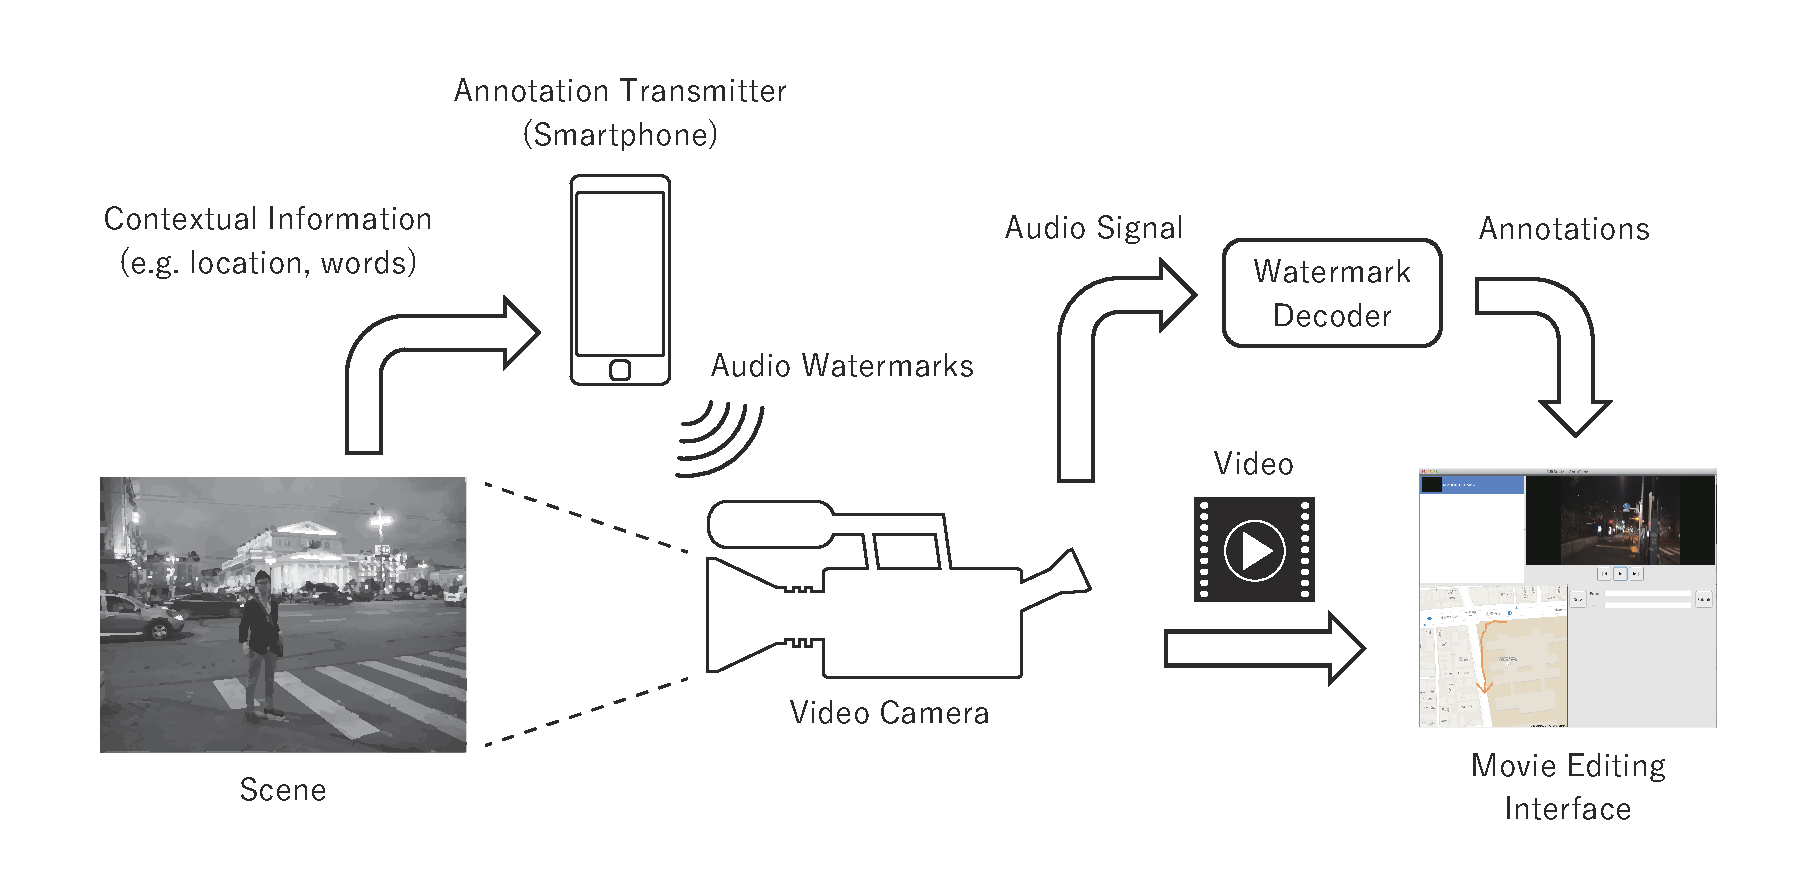
\includegraphics[width=150mm]{overview.pdf}
 \end{center}
 \caption{The schematic diagram of the system of AnnoTone}
 \label{fig:one}
\end{figure}

% AnnoToneのシステムは
% 1. アノテーションを生成するプログラム
% 2. アノテーションからWatermarkを生成するプログラムコンポーネント
% 3. Watermarkデコードを行うプログラムコンポーネント
% 4. アノテーションをもとに動画編集機能やUIを提供するプログラム
% によって構成される
The system of AnnoTone consists of four kinds of software components, those are watermark generator, watermark decoder, annotation interface and movie editing interface.
To guarantee the extensibility, we designed the system so that two interfaces can be implemented easily to realize new use of annotations using shared components for dealing with watermarks.

\section{Annotation Transmitter}
% 1と2でアノテーションレコーダーアプリを構成する
An annotation interface enables users to decide what to embed into a video as annotations, and sends them to a watermark generator to generate watermark signals representing them.
These two components comprise a smartphone application that transmits watermark signals from a back speaker of a smartphone to a microphone of a video camera.
The feature of the interface varies depending on the purpose of annotation.
It automatically makes annotations without any user operation if the purpose is to record a series of measured data like geolocation, otherwise it offers an user interface for users to explicitly embed annotations.

\section{Movie Editing Application}
% 3と4でビデオエディティングアプリを構成する
A watermark decoder and a movie editing interface constitute a software application that exploits embedded annotations for video editing.
The former take a video file imported from a video camera as an input and extracts annotations embedded into it as watermarks.
Extracted annotations are loaded into the movie editing interface, and offer its user a variety of functions for creating movie contents.

\if0
1. Audio Watermarking in Recording Time
	ほぼ変更なし
2. Preliminary Study for Modulating Method
	透かし仕様確定の事前研究として、二種類の変調手法を比較した
	可聴域を用いた高速伝達手法であるAcoustic OFDM
	FSKを拡張したオリジナルの手法であるAcoustic DTMF
	結果、後者のほうが今回の目的には適することが判明した
3. Acoustic DTMF in Inaudable Frequency Range
4. Packet Structure
\fi

\chapter{Watermarking Scheme}

\section{Audio Watermarking in Recording Time}
% 既存の音声透かし手法は適用できない
To enable embedding annotations for audio/visual editing in audio data, we owe fundamental idea for converting a digital data into an acoustic representation to existing audio watermarking techniques.
However, some significant differences between ordinary audio watermarking and embedding annotation for editing support make it difficult to apply the techniques straightforwardly to our purpose.

% ビデオ録画時に埋め込むので要請が異なる
In principle, the purpose of watermarking techniques is to add extra information like indication of intellectual property rights to existing contents by means of signal processing, therefore usually watermarking is conducted in the post-production stage.
On the other hand, our purpose requires embedding extra data in the audio track of a video while shooting it with a video camera. % to record annotations of a scene to support content creation.
It gives our recording-time watermarking distinctive technical requirements from basic audio watermarking techniques.

% 特殊なデバイスが使えない
Firstly, any requirements of extra equipment like specialized camera are not desirable.
Because our purpose is to support creators to make audio/visual contents, we should minimize hardware constraints and allow users to use our annotating technique with their favorite equipment for making content such as high-resolution camera and hi-fi audio recording system.
% リアルタイム重畳が必要
Secondly, host signal cannot be modified to embed data in our recording-time watermarking because host signal and annotation data are recorded simultaneously, unlike ordinary watermarking techniques take an existing content as a host signal to apply signal analysis and some modification for embedding data.
% Recently some techniques called {\it real-time watermarking} have been presented. Though these techniques realize real-time embedding of watermarking in contents, they are not suited for our purpose because they require extra equipment for digital signal processing.
% real-time watermarkingの話はrelated worksでしているので言及不要
% 耐攻撃性は不要
Thirdly, since our watermarks are used only in editing process, durability and transparency of watermarks are not very important, unlike ordinary watermarks are required to be hidden and resistant to elimination because most of them are embedded to contain essential information for preserving the content from abuses.
In contrast to ordinary watermarks, watermarks for editing support should be able to be eliminated completely after the editing process because they have no immediate value for consumers of contents.

% これらの条件から、host signalを書き換えられないので、加算的に合成することにした
% watermarkingに用いた周波数成分は上書きされて消えてしまうので、聴取に影響を与えないことが問題
According to these preconditions, we decided to use modulated tones of certain frequency bands for watermarking, making watermarking process significantly simple as generating encoded tones from digital data, transmitting them from a speaker near the microphone of a camera, and recording them as environmental sounds.
In this process, watermark signals and host signals are mixed in air like {\it sonic watermarking} by Tachibana. \cite{tachibana2003audio}
Removal of watermarks can also be simplified because eliminating certain frequency component from an audio signal can be done easily by applying an appropriate digital filter.
One problem is that, since certain frequency components of host signal would be overwritten by the watermark signals and also be eliminated in removing watermarks, we should select the frequency range not to spoil listening impressions.

% 前提条件
% ところで音声ファイルは44.1kHzで収録されるが、人は16kHzくらいまでしか聴こえない…
Most of common media formats use 44.1 kHz as their audio sampling rate, and virtually all video cameras and audio recorders can record sounds in this rate. It means that we can record media files that contain sounds with frequency up to 22.05 kHz with common equipment, since a discrete signal can contain sampled signals with frequencies lower than half of its sampling rate, according to the Nyquist-Shannon sampling theorem \cite{shannon1949communication}.
Human's hearing range is well-known to be between 20 Hz and 20 kHz, but some studies showed that absolute threshold of hearing (ATH) increases rapidly along with the frequency above 14 kHz and some people can not notice sounds above 18 kHz completely. \cite{:/content/asa/journal/jasa/86/4/10.1121/1.398698, ashihara2006hearing}
% in practice, sounds with frequencies higher than about 18,000 Hz cannot noticed by ordinary people unless they are informed the appearance of sounds in advance.
Because of these facts, digital data can be recorded in an audio sequence almost imperceptibly to human with common video cameras, if they are converted to audio signals with frequencies between about 18 kHz and 22 kHz.

% カメラに装着したスマートフォンをトランスミッタとして用いる
In our system named AnnoTone, annotation data are converted to inaudible modulated sounds in a frequency band between 17,600Hz and 20,000Hz, and transmitted to a microphone of a video camera from a speaker of a smartphone attached to the camera.
% GPSや加速度センサーをはじめとしたスマートフォンのセンサー群やタッチパネルUIの入力をアノテーションとして吹き込むことが出来る
A type of annotation data can vary depending on its usage, for example, values of various sensors carried on a smartphone such as GPS and accelerometer can be coded, and user inputs from user interfaces displayed on a touch panel of a smartphone are also available to make annotations.
% 異なるアノテーションは別々のアプリを用いて吹き込むが、透かし生成処理はライブラリ化されている
% これは実装の話だからここで書く必要はなさそう
% Different types of annotations are recorded using different smartphone applications, however core process of generating and extracting watermark signals from a digital data is provided as a software library therefore many applications could use it for annotating.


\section{Preliminary Study for Modulating Method}
% ビットレートの要件 ... double*3を入れるには200bpsは必須
Considering practical usage of annotations for content editing, we thought that in minimum 200 bps is required as the data rate of watermarking, because if a user wants to record a value of a sensor (e.g. GPS) consists of two or three double-precision floating-point number every second, 8 (bit/byte) * 8 (bytes) * 3 = 192 (bits) must be able to be embedded in one second.
% ヘッダや透かし間ギャップを考慮すると400bpsは欲しい
Taking an overhead from packet header/footer and required gap between watermarks for stability of decoding into account, at least 400 bps is desirable as the gross bit rate for our watermarking technique.

% 非可聴域を用いて変調を行うに当たって、我々は予備調査を行った
We conducted a preliminary study to choose appropriate method for modulating digital data into inaudible frequency range that satisfies this requirement.
In this study, we implemented watermark transmitters and demodulators for two modulation methods and roughly evaluated their performance by using them in real hardware setup.

% 一方はOFDM
The first method uses orthogonal frequency-division multiplexing (OFDM) to make full use of available bandwidth over 18 kHz, following the idea of Matsuoka's {\it Acoustic OFDM} \cite{matsuoka2008acoustic}.
% OFDMとは
OFDM is a specialized variety of frequency-division 
multiplexing (FDM) that uses multiple sub-carriers with different frequencies to transmit information in parallel.
A signal of OFDM is synthesized by composing signals of all sub-carrier waves.
% OFDMの特徴
In OFDM, carrier frequencies are selected in orthogonal, in other words, signals of sub-carriers are independent of and do not interfere each other.
This characteristic realize closer spaces between carrier frequencies and transmitting larger number of sub-carriers in certain bandwidth than ordinary FDM, therefore using OFDM increases bit rate of transmission.
% 用いた条件
In our preliminary study, eight sub-carriers with equally spaced frequencies between 17,900 Hz and 20,000 Hz were used to send octet bits in one signal, and each sub-carrier signal was modulated using differential binary phase shift keying (D-BPSK) in 100 bps (10 milliseconds per unit signal).
In total, gross bit rate was 800 bps in the condition, which satisfies the requirement mentioned above enough.

% 他方はDTMF
The other method also employs multiple sub-carriers with different frequencies to transmit information more than a bit in a unit signal, but it uses dual-tone multi-frequency (DTMF) technique for multiplexing.
A unit signal of DTMF is a composition of just two sinusoidal waves of different frequencies, and combination of the two frequencies represents the value of a signal.
Since the number of possible signal varieties of $n$-frequency DTMF is $_n C _2$, at most $\log_2 {}_n C _2$ bits can be sent in a signal.
% DTMFの特徴
In DTMF, the amount of information can be sent in a signal is smaller than OFDM if the number of sub-carriers are same, however, signal intensity of each frequency can be much stronger when that of composed signal is restricted by hardware constraints, because only two sub-carriers are composed simultaneously.
% 用いた条件
In this study, we used seven sub-carriers with equally spaced frequencies between 17,600 Hz and 20,000 Hz for DTMF. Since $_7 C _2$ is 21, 16 combinations among all pairs of seven frequencies were used to represent four bits per signal.
The length of a signal was set 10 ms, the same as that of first method.
In total, gross bit rate was 400 bps in the condition.

% 実験結果
As the result of the study, we found the first method with OFDM not suited for our purpose because of its worse embedding reliability besides its higher bit rate.
Extraction of watermarks is instable in the method due to the weaker intensity of each sub-carriers because of small output power of a speaker of a smartphone.
% 大きいスピーカーを使えば解決するが、今回の目的には適切ではない
However the embedding performance would be gained enough if a loud speaker with enough power could be available, using OFDM seemed not to be appropriate choice since small hardware constraint is required in our purpose.
% DTMFを使うことにした
In conclusion, we decided to use DTMF in our watermarking scheme appreciating its higher reliability.

% スペクトログラム
\begin{figure}[htbp]
 \begin{center}
  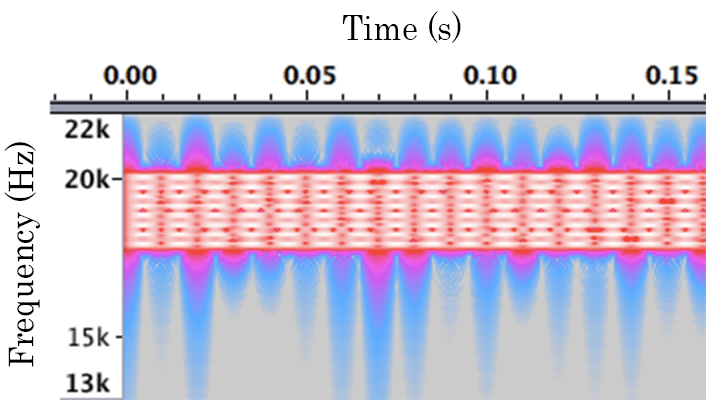
\includegraphics[height=35mm]{watermarking_ofdm.png}
  \hspace{5mm}
  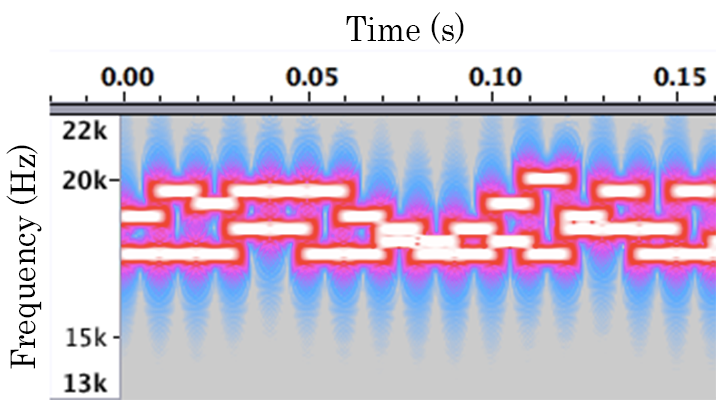
\includegraphics[height=35mm]{watermarking_dtmf.png}
 \end{center}
 \caption{Left: The spectrogram of a OFDM modulated watermark. Right: That of a DTMF modulated watermark.}
 \label{fig:watr_comp}
\end{figure}


%\section{Acoustic OFDM in Inaudible Frequency Range}
%% ビットレートの要件 ... double*3を入れるには200bpsは必須
Considering practical usage of annotations for content editing, we thought that in minimum 200 bps is required as the payload rate of watermarking, because if an user wants to record a value of a sensor (e.g. GPS) consists of two or three double-precision floating-point number every seconds, 8 (bit/byte) * 8 (bytes) * 3 = 192 (bits) should be able to embedded in one second.
% ヘッダや透かし間ギャップを考慮すると400bpsは欲しい
Taking overhead from packet header and required gap between watermarks for stability of decoding into account, at least 400 bps is desirable as the gross bit rate of our watermarking technique.

% 18kHz以上の帯域幅を有効に使うため、OFDMを採用した
To satisfy this requirement for bit rate, we adopt orthogonal frequency-division multiplexing (OFDM) as the modulation method to make full use of available bandwidth over 18 kHz, following the idea of Matsuoka's {\it Acoustic OFDM} \cite{matsuoka2008acoustic}.
% OFDMとは
OFDM is a specialized variety of frequency-division multiplexing (FDM) that uses a number of sub-carriers with different frequencies to transmit information in parallel.
In OFDM, carrier frequencies are selected in orthogonal, in other words, signals of sub-carriers are independent of and do not interfere each other.
This characteristics realize closer spaces between carrier frequencies and transmitting larger number of sub-carriers than ordinary FDM in certain bandwidth, therefore using OFDM increases bit rate of transmission.

% 17.9kHz~20khzの8並列で送ってる
AnnoTone uses 8 sub-carriers with equally spaced frequencies between 17900 Hz and 20000 Hz (17900 Hz, 18200 Hz, 18500 Hz, 18800 Hz, 19100 Hz, 19400 Hz, 19700 Hz, 20000 Hz) thus one byte can be sent in one parallel signal.
% サブキャリアのモジュレーションについて
Each sub-carrier signal is modulated using differential binary phase shift keying (D-BPSK) in 100 bps (10 milliseconds per unit signal).
D-BPSK represents binary data in a series of unit signals by phase shifting of certain frequency component.
A unit signal represents `` 1 '' when the phase of the signal is same as that of previous one, it represents `` 0 '' when the phase of the signal is shifted $\pi$ radians from that of previous one.
Using OFDM reduces computational cost of decoding significantly, enabling D-BPSK demodulation of each sub-carrier to be done in parallel without applying any filter such as band pass filter (BPF).
% 合計のビットレートは
In total, gross bit rate is 800 bps in our system, which satisfies the requirement mentioned above.


% 内容としては Packet Structure + DTMFのエンコード
\section{Acoustic DTMF in Inaudible Frequency Range} 
% DTMFに関して多少の詳細説明
A watermark of AnnoTone is modulated using DTMF technique mentioned above.
It can contain any kind of annotation data such as integer value, floating-point number, character string, and set of them.
Annotation data is serialized to a byte array and converted to a watermark packet structured as below.

% スペクトログラム
\begin{figure}[htbp]
 \begin{center}
  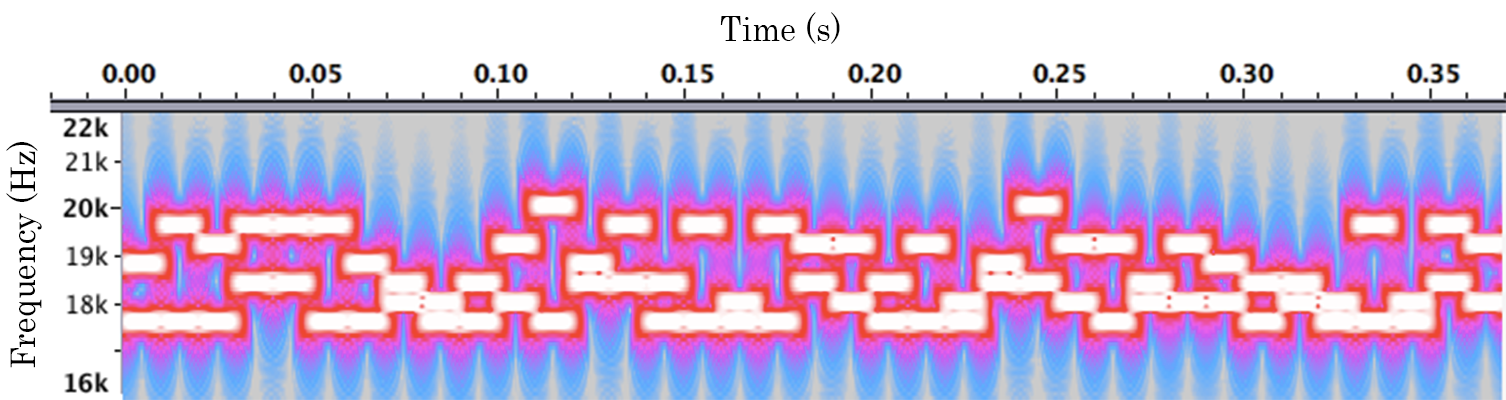
\includegraphics[width=120mm]{watermarking_spectrogram.png}
 \end{center}
 \caption{The signal spectrogram of a watermark packet that contains a geolocation data from GPS sensor.}
 \label{fig:watr_spec}
\end{figure}

% データフレームの定義
A data frame is the minimum unit of data representation in the watermarking scheme, and is a DTMF signal composed from two sinusoidal waves of the seven sub-carrier frequencies with length of 10 ms.
Since each data frame represents 4-bits information from 0 to 15, a data of one byte is encoded into two data frames.
The former frame of the two represents the lower four bits and the latter represents the higher four bits of a byte.

% パケット模式図
\begin{figure}[htbp]
 \begin{center}
  \vspace{5mm}
  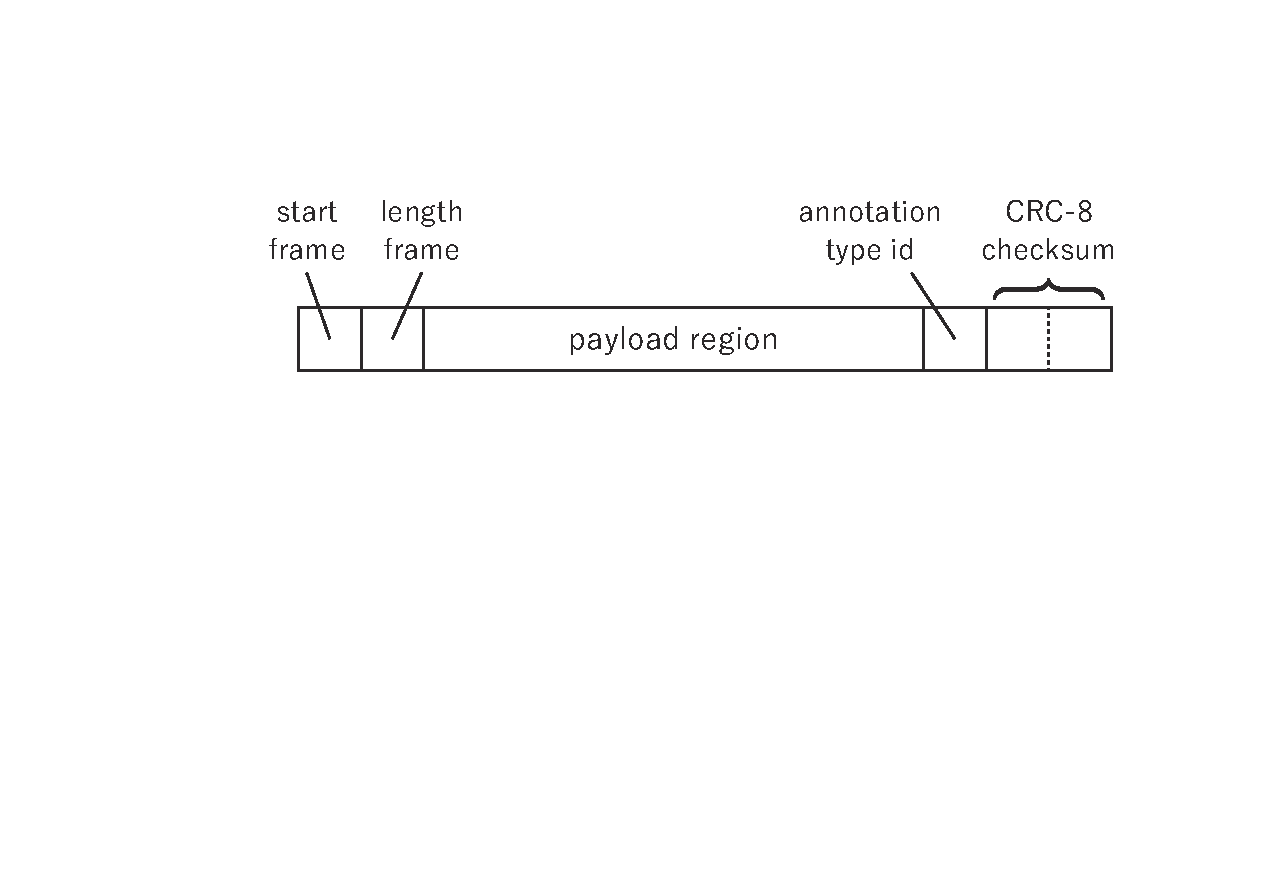
\includegraphics[width=120mm]{watermarking_packet.pdf}
 \end{center}
 \caption{Packet structure.}
 \label{fig:watr_pack}
\end{figure}

% パケットの定義
A packet is a set of several successive data frames representing an annotation data.
The data frame at the head of a packet is called start frame. It is fixed to represent ``2'', and it functions only as a sign of the start position of the packet. There is no special reason for choosing this number.
The second data frame specifies the length of payload region following it to be $ 2^n $ bytes where $n$ is the value of this data frame. It enables a payload size to vary depending on the type of an annotation. Consequently, the size of a packet can also vary.
From the third data frame, a payload region containing the body of an annotation data starts and continues for the length specified in the second data frame.
Multi-byte data such as an integer values are ordered in little endian, and multiple data are arranged in their original order in a payload region.
For example, an array of two short integer values \{0x1234, 0x5678\} would be arranged in a payload region as \{4, 3, 2, 1, 8, 7, 6, 5\}.
The data frame after the end of a payload region represents the annotation type id from 0 to 15 to distinguish multiple kinds of annotations embedded in one media file.
An annotation type id for a watermark can be decided arbitrarily by annotating applications.
A packet ends with two data frames representing the CRC-8 checksum of the packet for error detection in decoding. The polynomial for calculating CRC-8 checksum is $x^8 + x^7 + x^6 + x^4 + x^2 + 1$.


\chapter{Implementation}

\section{Overview}
% 4つのコンポーネントで出来ている
The system of AnnoTone consists of several software components, those are watermark generator, extractor, eraser, annotation interface and movie-editing interface.
% annotation transmitter
An annotation interface enables users to decide what to embed into a video as annotations, and sends them to a watermark generator to generate watermark signals representing them.
These two components comprise a smartphone application that transmits watermark signals from a speaker of a smartphone to a microphone of a video camera.
% extractor and editing interface
Annotations embedded in a video recording are extracted by the watermark extractor and loaded into the movie-editing interface, and offer its user a variety of functions for creating movie contents.
% erase
Embedded watermarks can be removed from an audio track of a video by the watermark eraser when they become unnecessary after the editing process is finished.

\begin{figure}[htbp]
 \begin{center}
  \vspace{5mm}
  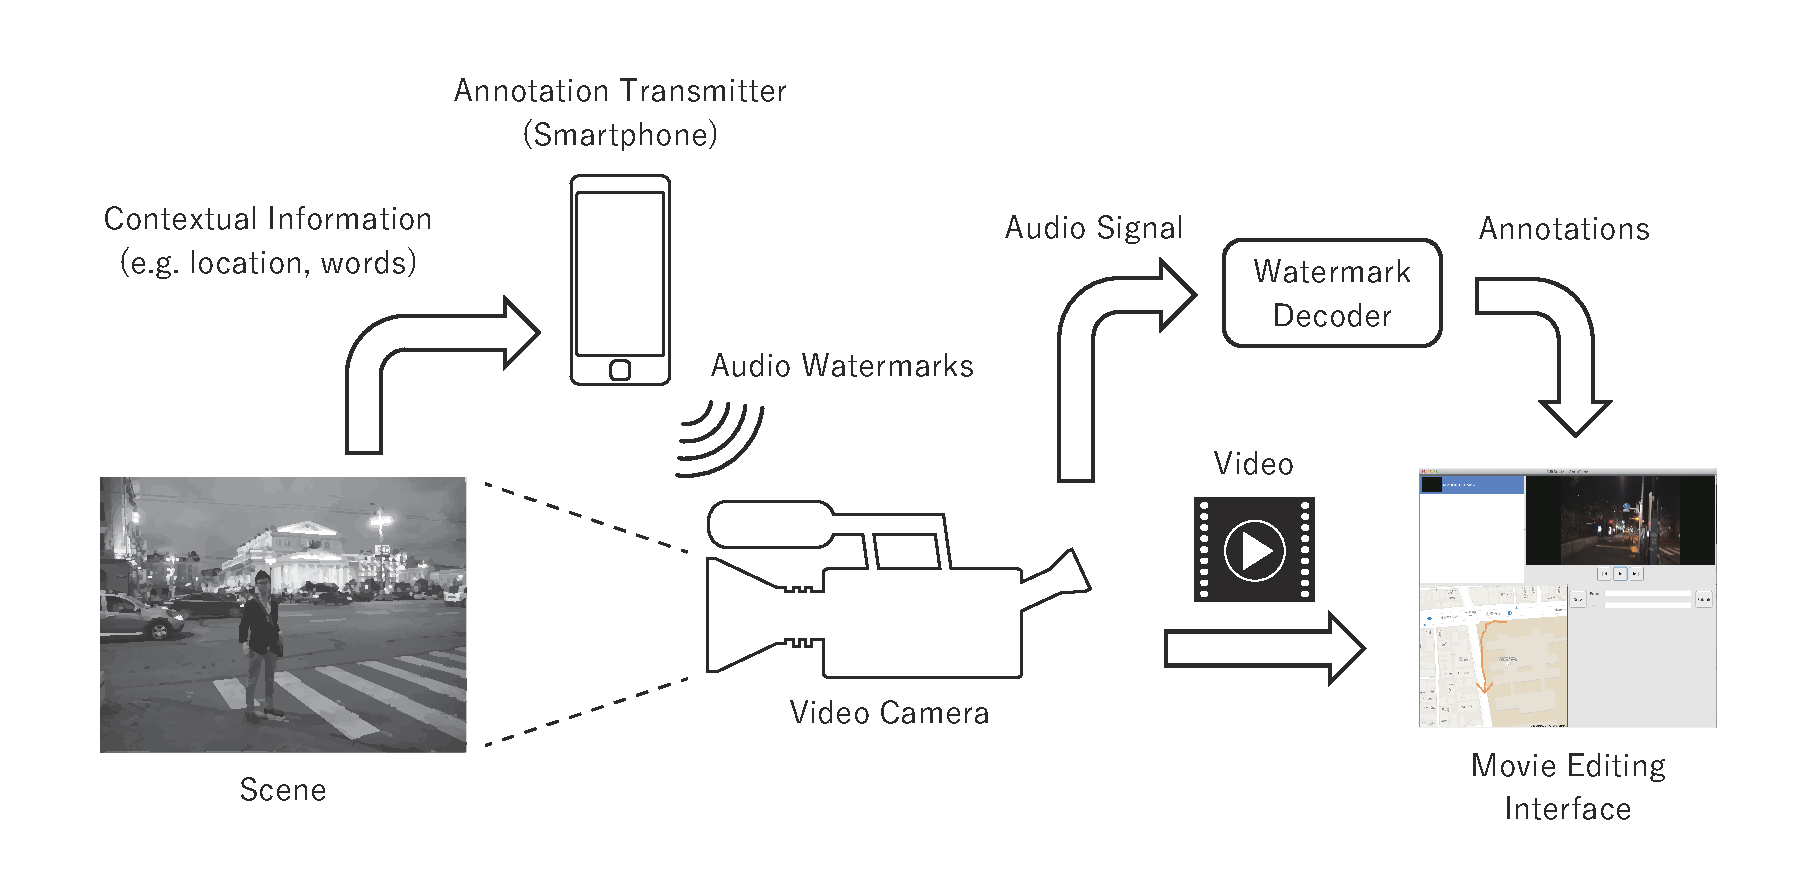
\includegraphics[width=135mm]{overview.pdf}
 \end{center}
 \caption{The schematic diagram of the system of AnnoTone}
 \label{fig:one}
\end{figure}

% 汎用性
Because we thought that our annotation method should be available for various kinds of applications depending on the purposes of users, watermark generator and extractor are provided as shared software libraries, and anyone can create a new application that exploits the value of annotations for movie-editing by only implementing the two interfaces.
% 以下本章では、この共有ライブラリおよびeraserの実装についての説明を行う。
We describe implementation of these shared libraries and watermark eraser in the rest of this chapter.
% インターフェイスはアプリケーションごとに内容が異なるので、後ほどApplicationsの章で解説する。
Because the two interfaces are application-dependent, we give detailed information about their examples in chapter 6, separately.

\section{Watermark Generation}
% 共通で使用できるAndroid用ライブラリを作成した
% ライブラリは次のようなアルゴリズムを使用している
In the system of AnnoTone, watermark signals are generated and transmitted from a smartphone.
We implemented a software library that provides essential functions for watermarking using following algorithm. % that can be used to create android applications for AnnoTone 

% 入力データに対してどのように処理を行うか
% annotation -> byte array -> packet -> wave data
% 位相変化時の低周波成分ノイズ発生を抑えるために窓関数を掛ける
First, an annotation of any kind of data (e.g. GPS position, a situation of ball game) is serialized to a payload, an array of 4-bits data following the arrangement manner mentioned in the previous chapter.
Secondly, a data stream of a packet is generated from the payload by calculating CRC-8 checksum.
Thirdly, DTMF-modulated pcm wave is generated using following formulae.

$s(t, m)$ is the sample value of the m-th sub-carrier at timestamp $t$ (s) counted from the beginning of the wave. $f(m)$ is the frequency (Hz) of the m-th sub-carrier and $d(n)$ is the n-th 4-bits data of the payload.

\begin{align}
s(t, m) = w( 0.5 \cdot a(m, d(\lfloor \frac{t}{0.01} \rfloor)) \cdot \sin{(2 \pi t \cdot f(m))} )
\end{align}

$a(m, x)$ is DTMF encoding function defined as the $(m, x)$-th element of below table.
(Blank means zero)

\begin{table}[ht]
\begin{center}
	\begin{tabular}{|c||c|c|c|c|c|c|c|c|c|c|c|c|c|c|c|c|} \hline
		  & 0 & 1 & 2 & 3 & 4 & 5 & 6 & 7 & 8 & 9 & A & B & C & D & E & F \\ \hline \hline
		7 &   &   &   &   &   & 1 &   &   &   &   & 1 &   &   &   & 1 &   \\ \hline
		6 &   &   &   &   & 1 &   &   &   &   & 1 &   &   &   & 1 &   &   \\ \hline
		5 &   &   &   & 1 &   &   &   &   & 1 &   &   &   & 1 &   &   & 1 \\ \hline
		4 &   &   & 1 &   &   &   &   & 1 &   &   &   & 1 &   &   &   & 1 \\ \hline
		3 &   & 1 &   &   &   &   & 1 &   &   &   &   & 1 & 1 & 1 & 1 &   \\ \hline
		2 & 1 &   &   &   &   &   & 1 & 1 & 1 & 1 & 1 &   &   &   &   &   \\ \hline
		1 & 1 & 1 & 1 & 1 & 1 & 1 &   &   &   &   &   &   &   &   &   &   \\ \hline
	\end{tabular}
\end{center}
\end{table}

$w(x, t)$ is an envelope filtering function to reduce the occurrence of low frequency noise at borders between two data frames.

\begin{align}
w(x, t) &= (0.5 - 0.5\cos{( 2 \pi \frac{t \bmod 0.01}{0.01} )}) ^{0.8}
\end{align}

Finally, watermark signal $x(t)$ to transmit is generated by mixing all sub-carrier signals as $ x(t) = \sum^{7}_{m=1} s(t, m) $.


\section{Watermark Extraction}
% watermarkデコードのアルゴリズム
Since DTMF modulation can be regarded as a special variety of frequency-shift keying (FSK), watermarks of AnnoTone embedded in media files can be extracted using common demodulation methods for FSK.
We implemented a extractor library using following algorithm, which could be used for creating applications utilizing annotations for content editing.

% 結果
\begin{figure}[htbp]
 \begin{center}
  \vspace{5mm}
  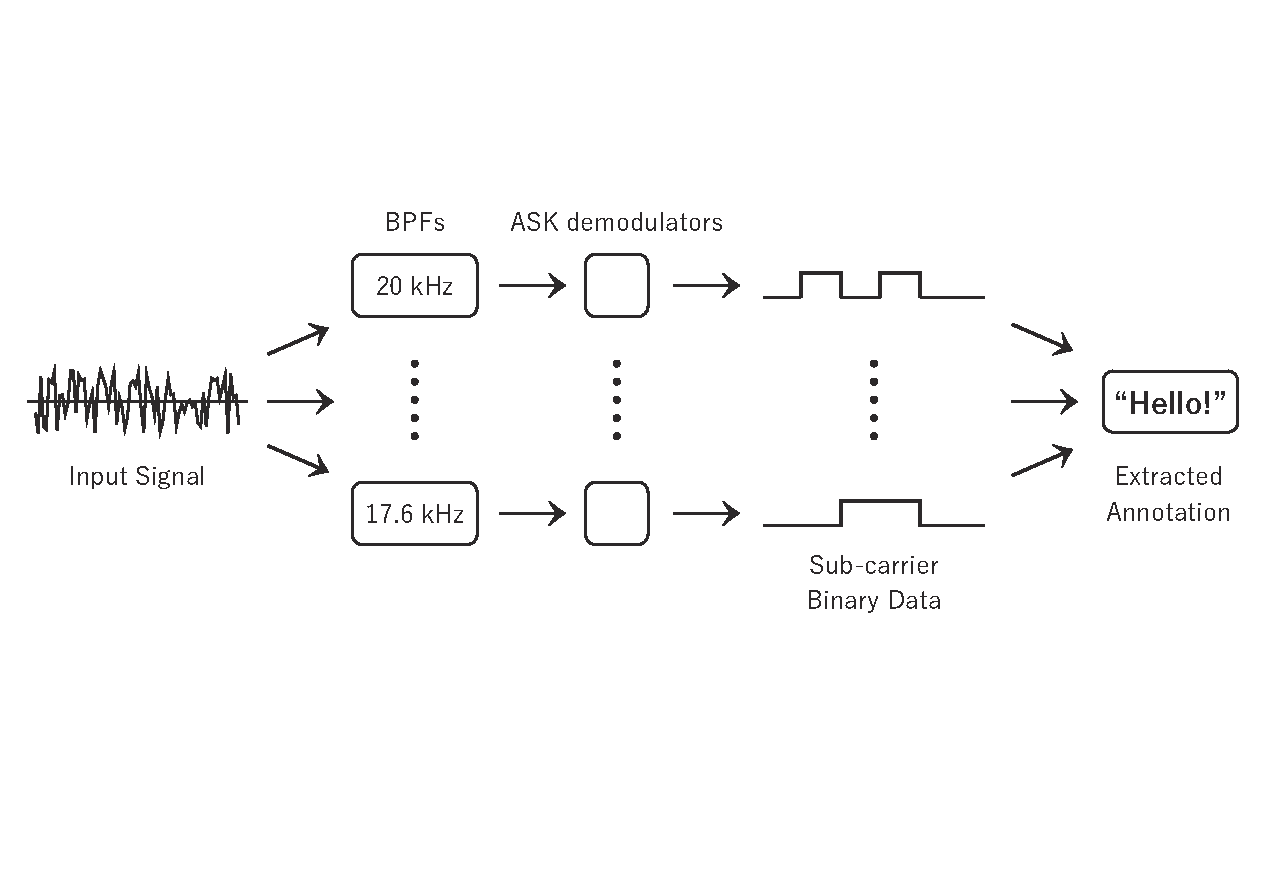
\includegraphics[width=130mm]{implementation_decode.pdf}
 \end{center}
 \caption{A schematic diagram of decoding algorithm.}
 \label{fig:impl_decd}
\end{figure}

% 形式を変換
Firstly, any kind of input file such as MPEG-2 format video is converted to pcm (.wav) file with 16 bit / 44.1 kHz sampling format using an external audio/video converter such as ffmpeg \cite{ffmpeg}.
% 各周波数ごとにBPF
Secondly, input signal is filtered by band-pass filters (BPFs) for each sub-carrier frequencies to extract each sub-carrier signals.
In our implementation, BPFs are designed as 199-tap finite impulse response filters.
After applying BPFs, binary states of each sub-carriers can be decided by a method for demodulating amplitude-shift keying (ASK).
% サンプル値の絶対値を取ってLPFに掛けてエンベロープを計算 
Thirdly, approximate envelopes of each sub-carrier signals are calculated by applying low-pass filter to them after taking absolute values of samples.
% エンベロープを簡単に2値化する
Fourthly, each envelope of frequency $f$ is binarized by a threshold $t(f)$ adaptively decided by the maximum value $max(f)$ and minimum value $min(f)$ of it as follows.

\begin{align}
t(f) = 0.9 \cdot min(f) + 0.1 \cdot max(f)
\end{align}

% タイムスタンプごとにDTMFデコードする
After this binarization, 4-bits values at each timestamp are scanned using the DTMF-encoding table mentioned above.
If the number of active sub-carriers is fewer than two, 4-bits value is regarded as invalid  at the timestamp, and if more than two sub-carriers are active, two sub-carriers with highest envelope values at the timestamp are used to decide the 4-bits value.

% 最後にパケット探索する
Finally, annotation packets are decoded from the scanned 4-bits value stream.
A start frame of a packet is identified by successive appearance of fixed value ``2'' for the half-length of a data frame.
After identifying a start frame, values for each data frames in the packet are decided by seeing 4-bits values at intervals of 10 ms.
% 続けて読み込むパケット長はlength frameから決定する
The number of data frames to read continuously is decided from the second data frame of the packet.
% 1パケット読み込み終わったらCRC-16チェックし、誤り検出されなかったら透かしとして確定する
After reading all data frames of a packet, it is extracted as an annotation if it passes CRC-8 error detection.

\section{Watermark Erasure}
% extractionと同じ方法で透かしの存在する区間を確認する
% 透かし区間に対して各周波数帯のBEFを適用する
Because watermark are embedded in a limited frequency range, their signal intensities can be decreased using an appropriate filter that attenuates signals of the sub-carrier frequencies.
We implemented a watermark deletion program that simply applies low-pass filter with 17,000 kHz cut-off frequency to an input sound.
% 下記の実験に示すようにこの簡単な手法でほぼ完全に不可聴にできるが、デコードは可能であった
As demonstrated in the following chapter, this elimination method can make watermarks inaudible almost completely, however part of them can be decoded even after the elimination.
% 完全に情報を復元できないようにwatermarkを消すには、この成分を完全に除去する必要がある
In order to completely remove watermark signals from a file, we can do downsampling to get rid of the information of sub-carriers at the expense of listening quality.
% サンプリングレートを落としたりmp3にすると消えることがわかっているが、音質は落ちる
Additinaly, we found that compressing an audio file to a MP3 format with a bit rate below 160 kbps removes high-frequency components almost completely from the signal, therefore this also can be used to delete watermarks from a media file.


\chapter{Evaluations}

\section{Environments and Setup}
% 実用性を示すために一連の性能評価を行った。
To show the practicality of the proposed technique, we conducted a series of performance evaluations on our watermarking scheme.
It consisted of three objective evaluations to prove the robustness of the scheme in actual situations, and a user testing to judge that our method can be used without spoiling the listening impression.

% 提案手法の有用性を検証するために、リアルなハードウェア構成でwatermarking schemeの性能評価実験を行った
In these evaluations, we used a prototypical hardware setup assuming real usage.
% ハードウェア構成
% 家庭用ビデオカメラ(型番)とスマートフォン(型番)で構成され、スマートフォンはカメラの外部マイクに固定する
This consisted of a consumer-use digital camcorder (SONY NEX-VG30H) and a smartphone (SAMSUNG Galaxy S) to generate and transmit watermarks.
The phone was attached to the microphone unit of the camera.
% カメラ設定
Movies were recorded in the conventional MPEG-2 format using standard definition image quality, and sound was recorded in 2ch stereo PCM format.
Default values were used for the other configurations of the camcorder.
% スマートフォン設定
Annotation transmitter applications were installed on the smartphone.
The audio output level of the phone was set an appropriate value empirically decided.

\begin{figure}[htbp]
 \begin{center}
  \vspace{5mm}
  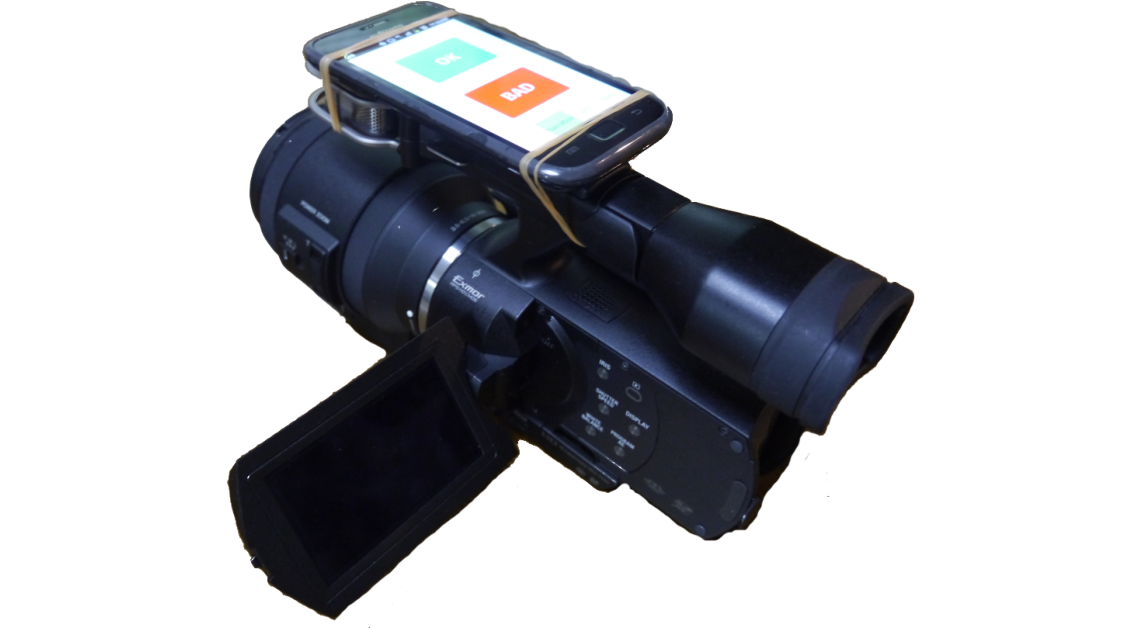
\includegraphics[width=90mm]{evaluation_environment.pdf}
 \end{center}
 \caption{The hardware setup used in the performance evaluations.}
 \label{fig:eval_hard}
\end{figure}


\section{Reliability of Embedding}
% 本手法が実用に適することと性能限界を示す ... 埋め込みのreliabilityを評価した
% reliabilityとは、現実的な状況で埋め込まれたwatermarkが十分に解読できることの保証である
To verify proposed watermarking method to be feasible and to show the performance limit of that, we evaluated the reliability of watermark embedding, guarantee that watermarks embedded in practical situations can be detected correctly with adequate certainty.
% 様々な設定で透かしの収録を行い、デコード可能なwatermarkの割合(CDR)を測定した
We recorded videos embedding watermarks with various watermarking settings, and measured the correct detection rates (CDRs) of watermarks in each.
% 実際の映像撮影は様々な場面で行われ、環境音の現れも多様であるため、以下の実験はsilent/public/rock/electronicという4つの音響条件下でそれぞれ行い、いずれの状況でもreliabilityが確保されるかを試した
Generally, videos are recorded in diverse situations; therefore characteristics of environmental sound also vary depending on them.
Taking it into consideration, we conducted following experiments in four different environmental settings, those are silent room, public space, playing rock music and playing electronic music, to see that embedding reliability of our method is retained in any situations.

% まず、どの程度の量のデータを安定に埋め込めるかを評価するため、bit rateを色々変化させてCDRを測定した。
% bit rateはdata frameが短いほど高くなるので、data frame長を6ms(666bps)から10ms(400bps)まで1ms刻みで変化させて5種類の実験を行った
% 各watermarkはランダムな16bytesのデータで、3秒おきに100個のwatermarkを連続で埋め込んでデコードした
Firstly, we measured CDRs changing the data rate of watermarking to evaluate how much data can be embedded per unit time stably.
Since the length of a data frame decides the data rate of watermarking, we changed it from 6 ms to 10 ms at 1 ms intervals.
6 ms length of a data frame corresponds to about 666 bps data rate, and 10 ms corresponds to 400 bps.
For each data frame lengths and environmental settings, one hundred watermarks with 16 bytes payloads were embedded at 3 seconds intervals, and the correctly detected watermarks were counted using our watermark decoder after recordings.
Figure \ref{fig:eval_reli_btrt} shows the measured CDRs in each condition.
This result shows that enough reliability can be gained in any recording environments if the data frame length is set 10 ms.
CDRs dropped rapidly as data frame length decreased below 10 ms, especially in the environment with electronic music.
It is probably due to the high-frequency tones contained in the music that confuse watermark detector.
From the result, we concluded that 10 ms was the optimal value for the length of a data frame.

% bit rate依存のreliability変化
\begin{figure}[htbp]
 \begin{center}
  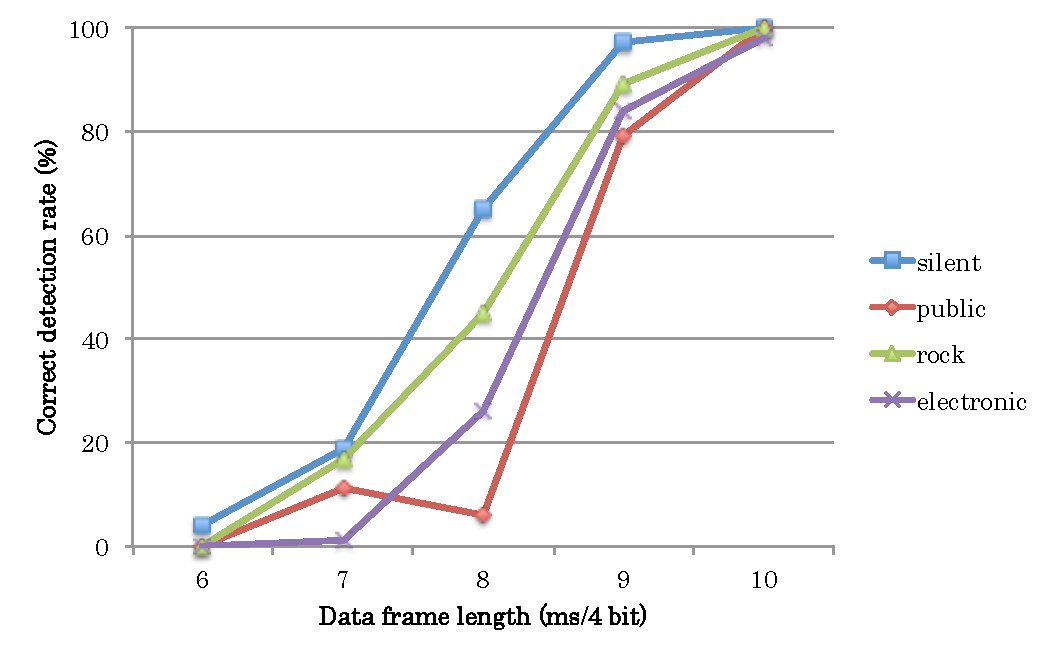
\includegraphics[width=120mm]{evaluation_reliability_bitrate.pdf}
 \end{center}
 \caption{The correct detection rates (CDRs) at variable data rates.}
 \label{fig:eval_reli_btrt}
\end{figure}
% 結果は〜

% 次に、安定に埋め込めるパケットの大きさを評価するため、payload長を色々変化させたpacketを埋め込んでCDRを測定した。
Secondly, we conducted a similar experiment changing the payload length of a packet to confirm that even a large data can be embedded as a watermark stably.
% 8, 16, 32, 64, 128 bytes の5条件
In this experiment, one hundred watermarks with a certain payload length from 8 bytes to 128 bytes were recorded in a video, and the CDR was measured later.
% data frame lengthは10msに固定
The data frame length of watermarks was fixed 10 ms.
% 結果
The result shown in Figure \ref{fig:eval_reli_pyld} demonstrates that CDR was slightly decreased with payload length increasing, but retained above 95\% at all payload lengths and situations.
% 色々なタイプのデータを格納するのに利用することが出来る
This means that our method can be used to embed many kinds of annotations with various data sizes, from an integer value to a long string like a caption sentence.

% payload依存のreliability変化
\begin{figure}[htbp]
 \begin{center}
  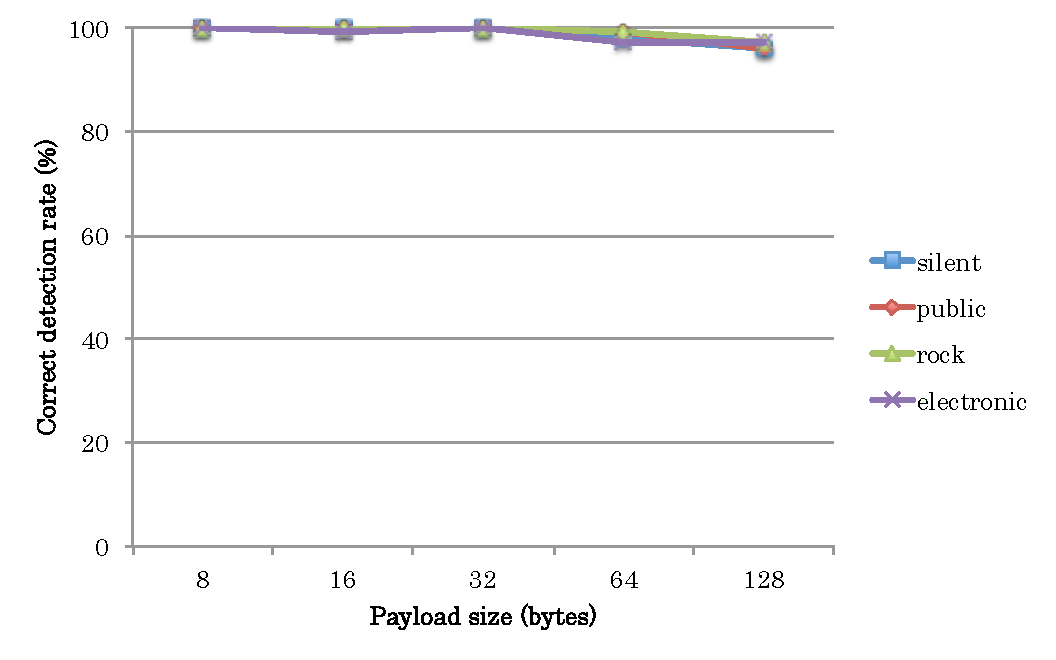
\includegraphics[width=120mm]{evaluation_reliability_payload.pdf}
 \end{center}
 \caption{The correct detection rates (CDRs) at variable payload sizes.}
 \label{fig:eval_reli_pyld}
\end{figure}

% しかし100%ではないので、何らかの冗長化機構をプロトコルに組み込むことを考えても良いかもしれない
However 100\% CDR is not guaranteed always in principle, these two experiments showed that AnnoTone's watermarking technique has adequate reliability for various usage in diverse recording situations.
If more accurate CDR was needed in any usage, we could append an error correction mechanism to our watermarking scheme at the expense of data rate.


\section{Durability against Audio Format Conversion}
% 編集の過程で形式変換はよく行われるので、この過程で保たれる必要がある
Audio format conversions are frequently applied to media files during movie authoring.
To assure embedded annotations to be available through a whole authoring process, it is important that watermarks are kept detactable after format conversions.
% 変換後に保存された透かしの割合を計測することで強度を測定した
We evaluated the durability against conversions by measuring the propotion of preserved detactable watermarks on videos after a variety of format conversions.
% 10個のdetactableなwatermarkを含むwavファイルを圧縮したものにデコードを試みた
In this evaluation, an uncompressed audio file with ten detectable watermarks was converted to a compressed format using an audio encoder program and then watermark detection was applied to the converted file.
% 形式
MP3, Ogg Vorbis and AC-3 (also known as {\it Dolby Digital}) were selected as the compression algorithms because of their high popularities.
% 品質
For each formats, compressions were applied in four bit rate settings between 128 kbps and 320 kbps to examine the needed compression quality for preserving watermarks in each formats.
% 5種類のファイルに関して実験した
We measured the correct detection rates for five different audio files and calculated the averages and standard deviations for each format and quality settings.

% 結果
\begin{figure}[htbp]
 \begin{center}
  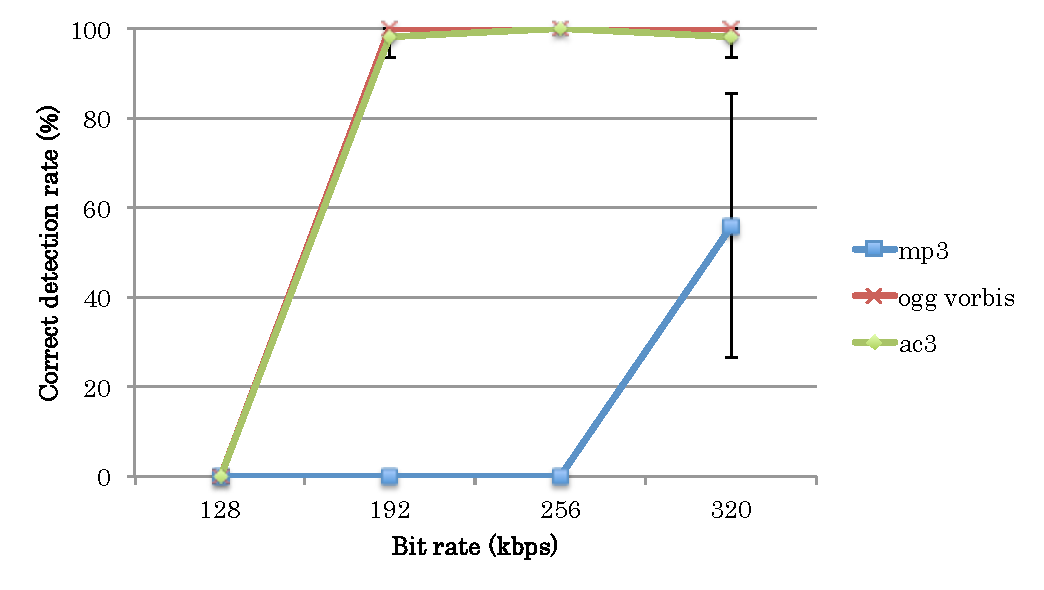
\includegraphics[width=120mm]{evaluation_conversion.pdf}
 \end{center}
 \caption{Average CDRs after format conversions for each compression settings.}
 \label{fig:eval_conv}
\end{figure}

According to the result shown in Figure \ref{fig:eval_conv}, watermarks can be preserved almost completely after a format conversion with Ogg Vorbis or AC-3 format and modest quality setting (over 192 kbps).
It suggests that our method can be used in practical movie authoring process since obviously satisfying these format requirements is not difficult.
% 一方でMP3が使えない
On the other hand, MP3 seems not suited for preserving watermarks even in a high bit rate setting, due to the characteristics of the compression algorithm.
This fact means that recording instrument limited to store audio data in MP3-compressed format, such as several kinds of IC recorders and inexpensive video cameras, can not be used for embedding watermarks of AnnoTone.
% まとめが欲しい?


\section{Transparency}
% 被験者実験によってtransparencyを評価した
We evaluated the transparency, or inaudability for human, of watermarks by a subjective experiment.
In this experiment, five participants are asked to listen to recorded sounds with embedded watermarks from a headphone and push a button when they notice unnatural noise.
For every participant, the output volume was set a constant value that he/she usually uses to listen to a music.
After that, the number of noticed watermarks is counted for each participant and sound.
We regarded a watermark to be noticed if a participant pushed the button within a second after the watermark is played.
% 4つの環境で録音された
Same as the experiments mentioned above, we tested the transparency in four environmental situations respectively to see the change of results depending on situations.
% elimination掛けたり掛けなかったり
In order to evaluate the effect of our watermark deletion program, we prepared two recordings for each situation, one is applied watermark deletion and the other is not.
In total, we used eight recordings in this experiment.
% 音源の情報
Each recording is one minute long and contains ten watermarks with 16 bytes payloads at randomly selected positions.

% 結果
\begin{figure}[htbp]
 \begin{center}
  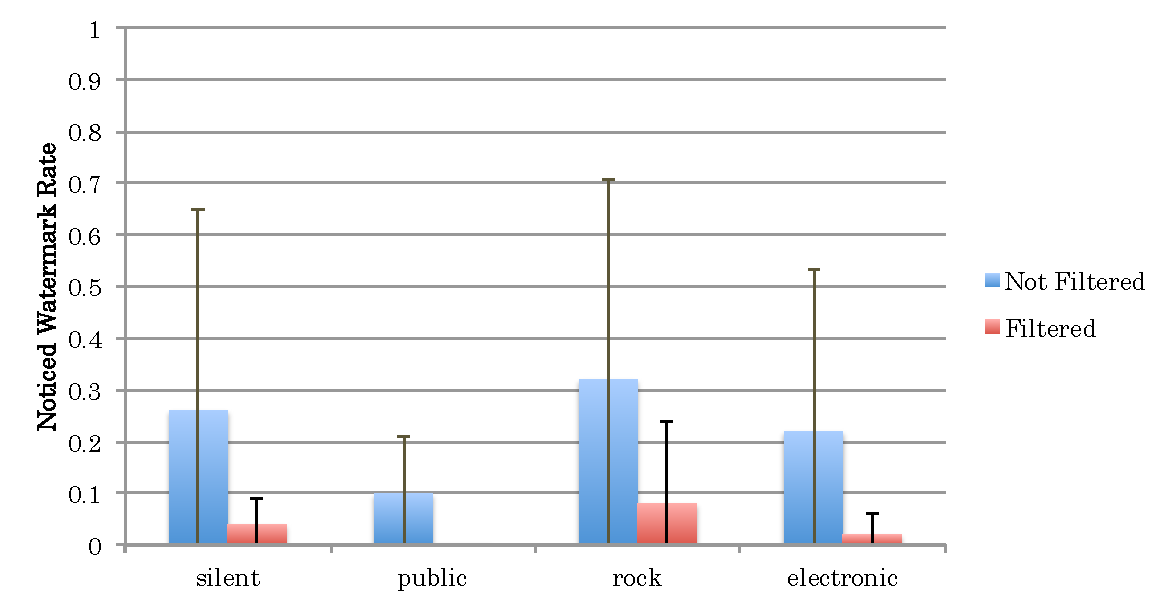
\includegraphics[width=120mm]{evaluation_transparency.pdf}
 \end{center}
 \caption{Mean rates of noticed watermarks for each conditions.}
 \label{fig:eval_tran}
\end{figure}

The result is shown in the graph above.
% notice rateはwatermark elimination以前からたかだか3割程度であって、
% 音源のqualityに大きな影響を与えていないと考えられる
Noticed watermark rates were at most 30 \% before being applied a watermark deletion in every situation.
% watermark eliminationを施した後では、ほとんど全く検知が不可能になっており、有効性が確認できる
After the deletion, the rates were much less than the source signals, and watermarks are virtually transparent.
These facts might indicate that our watermarking method can be used without decaying the quality of sound.
% また、notice rateには個人差が大きく、特に年齢が高い被験者はほとんど検知することが出来なかったが、これはよく知られた聴覚の衰えによるものであろう
Interesting point is that the difference of noticed watermark rates between indivisuals is very large, and young participants tend to notice more watermarks than mature ones.
This may be due to the universal high frequency hearing loss accompanied by aging.

\chapter{Applications}

To demonstrate the usefulness, we created three applications with our annotation technique that realize novel interaction styles in movie making process.

\section{Recording-time Editing}
% ポストプロダクション段階で、エディターはカットやエフェクトなど様々な作業をしなくてはならない
In the post-production stage, a movie creator should do a lot of operations such as cutting scenes with mistakes, removing unexpected noise, applying audio and visual effects at appropriate timings, {\it etc}.
% それらの作業のために必要な情報は撮影時に発生するが、逐一ビデオと別途記録するのは面倒である
Most of information needed for the process, such as when an actor appeared in a scene, are shown during the shooting, however, we cannot note all of them with ordinary equipment.

% AnnoToneを使えば、そういう情報を録画中に埋め込んでおいて自動編集に使える
Using AnnoTone, we can embed those kinds of information into a video in recording time, and conduct automatic editing after recording in accordance with the recorded annotations.
% 映像から失敗の部分を自動で切り取る、とても簡単なアプリケーションを作成した。
We created a very simple video-editing application as a example of such usage, that automatically cut sections with mistakes off from a video.

\begin{figure}[htbp]
 \begin{center}
  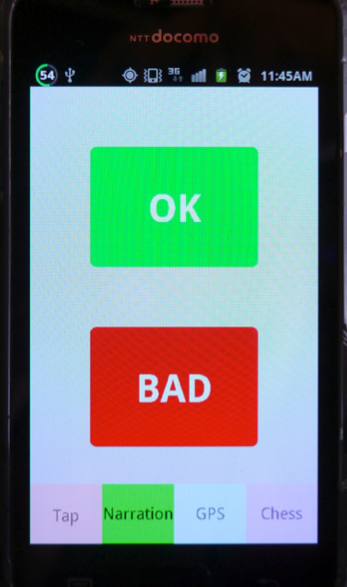
\includegraphics[height=70mm]{application_edit_app.png}
  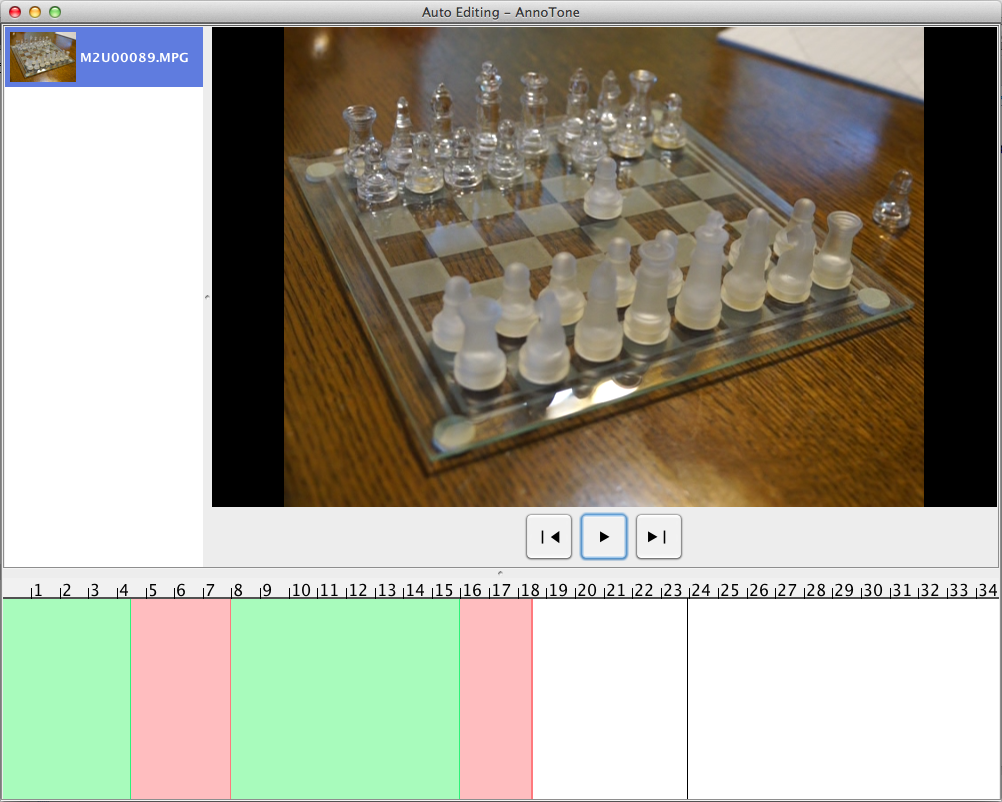
\includegraphics[height=70mm]{application_edit.png}
 \end{center}
 \caption{Left: The user interface of annotating application. Right: Automatic video cutting application.}
 \label{fig:appl_edit}
\end{figure}

% 使い方の説明
A camera operator repeatedly taps one of the two buttons displayed on the interface (Figure \ref{fig:appl_edit} Left) of a smartphone during shooting a video to embed annotations that indicate whether the recent performance was good or not.
After the shooting, video editing application detects the annotations and divides the video into a series of sections at the annotated points.
Each section is marked ``OK'' or ``BAD'' based on the annotation that follows it, and sections marked ``BAD'' are cut off from the video.
% Figureの説明
The user interface of the application is shown in Figure \ref{fig:appl_edit} Right.
Timeline of the loaded video is displayed in the lower part of the interface, and each section is colored depends on how it is marked.
Red colored sections are marked ``BAD'', and they are automatically skipped when the user playback the video in the movie player above.


\section{GPS-logging for Movie Editing}

% 動画は歩きながらあるいは乗り物に乗りながら撮影されることがあり、そうした動画では多くの場合各時点における位置情報がコンテンツにとって重要な意味を持つ
Sometimes a video is recorded with the camera user walking or riding on a vehicle.
In most cases of that kind of videos, location information at each moments of a video have significant meaning in making movie contents.
% 例えば自転車レースを記録した映像であれば、特定の難所を選手が通過するシーンだけを抽出したいといった需要がある
For example, in case of creating a documentary of a bike race, there is a large demand for extracting certain scenes in which riders are passing a dangerous spot.

\begin{figure}[htbp]
 \begin{center}
  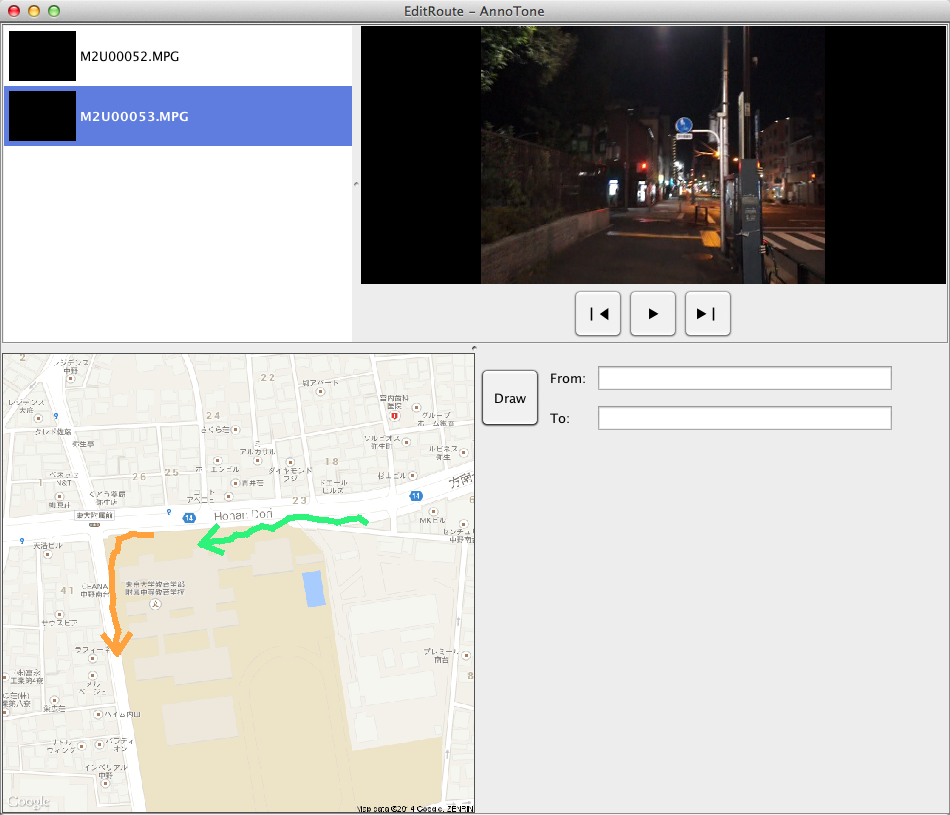
\includegraphics[width=100mm]{application_map.png}
 \end{center}
 \caption{The user interface of our geolocation-based video editor.}
 \label{fig:appl_map}
\end{figure}

% 我々は動画に周期的にglobal positionを埋め込むことで編集時に位置情報とタイムスタンプを対応付けられるようにするシステムを開発した
We created a system that embeds geolocation of the camcorder measured by a GPS sensor into a video in the intervals of a few seconds.
The path, or the series of geolocations associated with timestamps of a video is used to provide an user interface that enables geolocation-based video editing.
Using this geolocation-based system, user can interact with videos fully exploiting their spatial semantics and without paying extra attention on timestamps in a movie authoring process.

% UIの説明
Figure \ref{fig:appl_map} shows the appearance of the interface.
Loaded videos are listed on the upper left listview, and can be watched in the upper right video viewer.
Paths embedded in the videos are visualized in the map below as green and orange winding arrows. That of the selected video is colored orange.
User can seek a timestamp of a video at which the camera is in a certain place by double-clicking the corresponding part of the arrow of that.
If a user double-clicked a curved position of an arrow, the moment of a video at which the camera is turning a corner would be seeked.
% クリッピング
User can clip a needed scene from loaded videos by two location-based means in this system.
In the use of first means, a user draws a line that specifies the expected path of the extracted clip along exsting paths by his/her hand, then the desired scene is automatically clipped from loaded videos.
On the other hand, the second means only requires its user to specify the names of start and end positions of expected clip, like ``from Paris to London''.
The system automatically finds the geolocations of the two positions using Google Maps API \cite{googlemapsapi} and a section of a video that starts and ends with the specified geolocations.



\section{Automatic Caption Overlaying}

% ほとんどの映像作品は状況を説明するオーバーレイキャプションを持つ
% 例えば球技の試合映像なら得点状況、旅行番組であれば地図、オペラならば歌詞などである
Almost every movie contents have overlaid captions or images that describe situations and provide supplementary information.
For example, a record of a ball game has a caption about the score, some TV programs about traveling would have overlaid maps, and a movie of a concert may have captions of words of songs.
% キャプション作成やタイミングを合わせて合成することは手間が掛かる
Making such captions and overlaying them in appropriate timings is a laborious part of a movie authoring process.
% AnnoToneにより状況を録画時に埋め込んでおくことで、多くの作業を自動化出来るだろう
In some cases, creating and overlaying captions would be able to be automated by embedding contextual information into videos and utilizing them by AnnoTone.

\begin{figure}[htbp]
 \begin{center}
  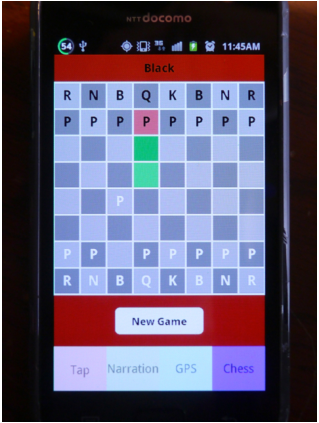
\includegraphics[height=60mm]{application_chess_app.pdf}
  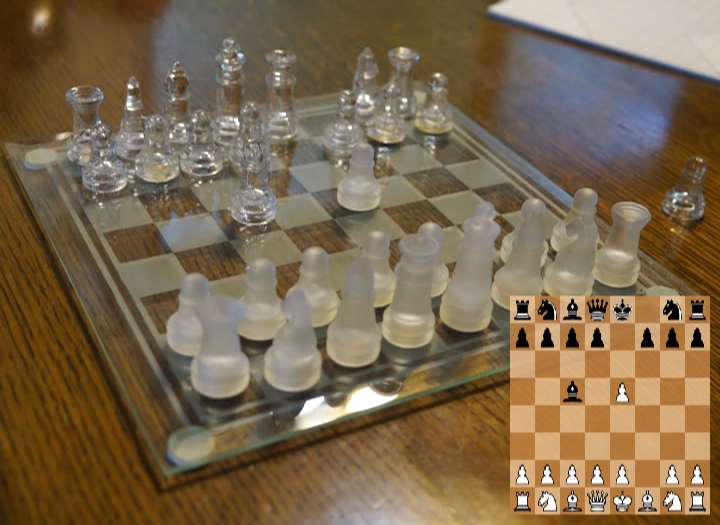
\includegraphics[height=60mm]{application_chess_movie.png}
 \end{center}
 \caption{Left: The user interface for annotating chess notes. Right: Movie overlaid with a chessboard by the system.}
 \label{fig:appl_chss}
\end{figure}

% 我々はチェスの記録映像を対象に、自動的に盤面状況を画面にオーバーレイするシステムを作成した。
As an illustration, we developed a system for chess movies that automatically overlay a video with an animation of a chessboard reflecting game progress using chess notes embedded in the video.
% アノテーションは、通常のプレイ時に棋譜を行うのと同様にプレイヤーまたはカメラマンが手動で行う
A camera person or players operate a smartphone application to embed the chess notes in a video, like recording notes in ordinary games.
The application provides a video game-like simple user interface (shown in Figure \ref{fig:appl_chss} left) presenting a chessboard to easily record a game.
Each chess note is generated as a record of standard Forsyth-Edwards Notation (FEN) therefore the notes embedded in a video represents all information of a game.
% ソフトウェアが棋譜が埋め込まれた動画を解析し、各時点での盤面の状況を画面右下にオーバーレイする
The system analyzes a video annotated with chess notes to calculate the states of chessboard at each timestamps and generate a series of overlay images as shown in Figure \ref{fig:appl_chss} right.

\chapter{Conclusions and Future Work}

conc.


%-------------------
%\bibliographystyle{plain} % 参考文献
\bibliographystyle{unsrt}
\bibliography{myref} %
%-------------------
\end{document}
